\setcounter{page}{1}
\clubpenalty=10000 
\widowpenalty=10000

%%%%%%%%%%%%%%%%%%%%%%%%%%%%%%%%%%%%%%%%
%      Шапка экспертной организации  
%%%%%%%%%%%%%%%%%%%%%%%%%%%%%%%%%%%%%%%%
%
\input   % Шапка 
{titul/оборудованиеАЭИип}  
%
%%   вопросы экспертизы
\subsection{Вопросы исследования}
%Заказчик поручает, а Исполнитель принимает на себя обязательство выполнить Заказчику  комплекс работ в виде автотехнических исследований автомобиля Mazda 6, VIN RUMGJ52\-6802007133 (дата начала гарантии 07.05.2018 г.), по следующим вопросам:
\begin{enumerate}
   
   \item
    Какие неисправности имеет двигатель \двигатель\, самоходной машины  KOMATSU   АВТОПОГРУЗЧИК  FG15T-20   2007 года выпуска, заводской номер 661043?
   
  \item
    Какова причина их возникновения?
   
  \item
    Причина выхода из строя  двигателя \двигатель\,  имеет производственный или эксплуатационный характер?
   
  \item
    Могли ли имеющиеся у  двигателя \двигатель\, неисправности возникнуть вследствие капитального ремонта?
  

  
%	\item  <<Связано ли повреждение панели рамки радиатора слева и брызговика с лонжероном переднего левого автомобиля ВАЗ 21099 с указанным ДТП?>>	
% \item  <<Что послужило причиной выхода двигателя автомобиля из строя?>>	   
%    \item  <<Является ли данная причина:
%\begin{itemize}
%        \item производственной, т.е. недостатком сборки и/или материала;
%        \item связанной с некачественным/несвоевременным обслуживанием автомобиля, включая ежедневный осмотр;
%        \item связанной с неразрешенными/недопустимыми переделками агрегата и/или его систем;
%        \item связанной с предыдущим ремонтом (если применимо);
%        \item эксплуатационной, т.е. возникшей по причине неправильной/ненормальной эксплуатации;
%        \item  естественным износом в соответствии с пробегом автомобиля?>> 
% 	\end{itemize}
%	
\end{enumerate}


\subsection{Термины и определения}
\begin{description}
    \item
    [Аварийные повреждения] -- повреждения, механизм образования которых определяется контактом с посторонними объектами, что привело к деформации или разрушению и к необходимости ремонта или замены составной части, или контактам с агрессивной средой, которая привела к необходимости ремонта (замены) составной части; %[1, часть II, п. 1.5].
    %	\item[Восстановительный ремонт]-- один из способов возмещения ущерба, состоящий в выполнении технологических операций ремонта КТС, действующий в сети торгово-сервисного обслуживания, созданной изготовителем этого КТС [1, часть II, п. 1.4].
    %	\item[Годные остатки] -- работоспособные, имеющие остаточную стоимость детали (агрегаты, узлы) поврежденного автотранспортного средства, годные к дальнейшей эксплуатации, которые можно демонтировать с поврежденного автотранспортного средства и реализовать.
\item
[Дата исследования]-- дата, на которую проводятся расчёты и используются стоимостные данные КТС, запасных частей, материалов, нормо-часа ремонтных работ;% [1, часть II, п. 1.5].
%    \item [Декоративные свойства лакокрасочного покрытия] -- способность лакокрасочного покрытия придавать окрашенной
%    поверхности заданный цвет и блеск
\item
[Дефект] -- это каждое отдельное несоответствие объекта требованиям, установленным документацией;
\item
[Исправное состояние (исправность)] -- состояние объекта, при котором он соответствует всем требованиям, установленным в документации на него;
\item
[Конструктивный отказ] -- отказ, возникший по причине, связанной с несовершенством или нарушением установленных правил и (или) норм проектирования и конструирования;
%\item
%[Защитные свойства лакокрасочного покрытия] --
%    Способность лакокрасочного покрытия предотвращать или замедлять
%    коррозию металлических или разрушение неметаллических поверхностей в
%    условиях агрессивного воздействия внешних факторов.
%\item
%[Лак] -- продукт, который после нанесения на поверхность образует твёрдую прозрачную 	плёнку, обладающую защитными, декоративными или специальными техническими свойствами.
%\item
%[Лакокрасочное покрытие (ЛКП)] -- сплошное покрытие, полученное в результате нанесения 	одного или нескольких слоёв лакокрасочного материала на окрашиваемую поверхность
%\item
%[Линия удара]-- линия, определяемая направлением вектора равнодействующего импульса сил, возникающих при контакте ТС при столкновении до прекращения взаимного внедрения деформирующихся при ударе частей. Положением линии удара на ТС определяются направление и величина момента импульса сил, возникающих при ударе, и, следовательно, направлением и интенсивность разворота ТС относительно центра масс после столкновения.  
\item
[Моделирование]-- исследование каких-либо явлений, процессов или систем объектов путем построения и изучения их моделей;
\item
[Малозначительный дефект] -- дефект, который существенно не влияет на использование продукции по назначению и ее долговечность;
\item
[Механизм отказа] -- процесс, который приводит к отказу
\item
[Морфологические признаки]-- признаки, отображающие внешнее и внутреннее строение объекта;
%\item
%[Недостаток лакокрасочного покрытия] -- отклонение лакокрасочного покрытия от 	требований нормативно-технической документации, образовавшееся в процессе нанесения и
%    формирования лакокрасочного покрытия (производственный недостаток)
\item
[Неработоспособное состояние (неработоспособность)] -- состояние объекта, в котором он не способен выполнять хотя бы одну требуемую функцию по причинам, зависящим от него или из-за профилактического технического обслуживания;
\item
[Неисправное состояние (неисправность) ] -- это состояние объекта, при котором он не соответствует хотя бы одному из требований, установленных в документации на него;
\item
[Неустранимый дефект] -- дефект, устранение которого технически невозможно или экономически нецелесообразно;
\item
[Отказ]  -–  событие, заключающееся в нарушении работоспособного состояния объекта;

\item[Пластичность] --  способность  материала
приобретать  необратимые  изменения  формы  под действием нагрузки;
\item
[Производственный отказ] -- отказ, возникший по причине, связанной с несовершенством или нарушением установленного процесса изготовления или ремонта, выполняемого на ремонтном предприятии;
\item
Производственный (технологический) дефект] -- дефект, вызванный нарушением установленной технологии изготовления детали, узла, агрегата;
\item
[Работоспособное состояние] -- состояние объекта, в котором он способен выполнять требуемые функции;
\item[Предел упругости ] -- свойство вещества, максимальная нагрузка, после снятия которой не возникает остаточных (пластических) деформаций;
\item
[ Прочность] --свойство материала сопротивляться разрушению под действием внешних сил;
\item
[Скрытый отказ] -- отказ, не обнаруживаемый визуально или штатными методами и сред-ствами контроля и диагностирования, но выявляемый при проведении технического обслуживания или специальными методами диагностирования;
%    \item[Срок эксплуатации КТС]-- период времени от даты изготовления (даты выпуска) КТС, до даты оценки (исследования), определяемой условиями задачи исследования (независимо от даты его регистрации и начала использования по назначению (эксплуатации))
\item
[Упругость] --  способность  материалов  изменять форму  под  действием  нагрузки  и  возвращаться  в исходное состояние после снятия нагрузки
\item
[Устранимый дефект] -- дефект, устранение которого возможно путем технического;
    обслуживания или ремонта
    
   
%    \item[Эмаль] -- жидкий или порошкообразный продукт, содержащий пигменты, который после
%    нанесения на поверхность образует непрозрачную плёнку, обладающую защитными,
%    декоративными или специальными техническими свойствами.
\item
[Эксплуатационный отказ] -- отказ, возникший по причине, связанной с нарушением уста-новленных правил и (или) условий эксплуатации;
\item
[Явный отказ] -- отказ, обнаруживаемый визуально или штатными методами и средствами контроля и диагностирования при подготовке объекта к применению или в процессе его применения;
\end{description}

\subsection{Задачи, поставленные перед специалистами}

Провести необходимые исследования и ответить на поставленные вопросы.

\subsection{Для производства исследования представлено}

\begin{enumerate}
    \item 	Автопогрузчик KOMATSU FG15T-20 заводской номер 661043;
    \item 	Светокопия свидетельства о регистрации машины  ВК № 384784,  на 1 листе;
    \item 	Светокопия паспорта самоходной машины и других видов техники ТС № 001742, на 1 листе;
    \item 	Светокопия акта № 441 от 04.10.2019 г., на 1 листе, составленного специалистом ИП Войтенко В.А.;
    \item 	Светокопия заказ-наряда № 252 от 04.10.2019 г., на 1 листе, составленного специалистом ИП Войтенко В.А.;
    \item 	Светокопия счета на оплату № 449 от 04.10.2019 г., на 1 листе, составленного специалистом ИП Войтенко В.А.;
    \item 	Светокопия письма исх. № 2 от 10.02.2020 г. генерального директора ООО «Логистик-Юг» (г. Краснодар);
    \item 	Светокопия заказ-наряда № 252/1/20 от 27.02.2020 г., на 1 листе.
\end{enumerate}
%
\addcontentsline{toc}{section}{Использованные нормативы и источники информации}
%
%\left( \addcontentsline{toc}{section}{Использованные нормативы и источники информации}

\subsection{Использованные нормативы и источники информации}
%
\begin{enumerate}
%	
%\vspace{-10mm}
%
%\item                                 
%Федеральный закон от 31 мая 2001 г. N 73-ФЗ \emph{О государственной судебно-экспертной деятельности в Российской Федерации} 
%
%\item
%Федеральный закон от 25.04.2002 N 40-ФЗ \emph{Об обязательном страховании гражданской ответственности владельцев транспортных средств} // Собрание законодательства РФ  06.05.2002, N 18, ст. 1720
%
%\item
%Федеральный закон от 28 марта 2017 г. N 49-ФЗ \emph{О внесении изменений в Федеральный закон "Об обязательном страховании гражданской ответственности владельцев транспортных средств} // Российская газета - Федеральный выпуск №7234 (68)
%
%
%
%\item 
%Махнин\,Е.\,Л., Новоселецкий\, И.\,Н., Федотов\, С.\,В. \emph{Методические рекомендации по проведению судебных автотехнических экспертиз и исследований колесных транспортных средств в целях определения размера ущерба, стоимости восстановительного ремонта и оценки} // --М.: ФБУ РФЦСЭ при Минюсте России, 2018.-326 с.  ISBN 978-5-91133-185-6
%
%\item  «Исследование автомототранспортных средств в целях определения стоимости восстановительного ремонта и оценки» (Методические рекомендации для судебных экспертов, утверждено  научно-методическим советом РФЦСЭ 13 марта 2013 г., протокол №35.), Минюст России, 20013г.
%%
%\item  Судебная автотехническая экспертиза. Институт повышения квалификации Российского Федерального Центра Судебной Экспертизы, М. 2007.
%
%\item
%Положение Банка России от 19 сентября 2014 года № 432-П \emph{О единой методике определения размера расходов на восстановительный ремонт в отношении повреждённого транспортного средства} // Вестник банка России, № 93 (1571). Нормативные акты и оперативная информация
%Центрального банка Российской Федерации. Москва, 2014
%
%\item
%Положение ЦБ РФ от 19 сентября 2014 года №433-П \emph{О правилах проведения независимой технической экспертизы транспортного средства} // Вестник банка России, № 93 (1571). Нормативные акты и оперативная информация Центрального банка Российской Федерации. Москва, 2014
%
\item 
Технический регламент Таможенного союза \emph{О безопасности машин и оборудования} (ТР ТС 010/2011), утвержденный решением Комиссии Таможенного союза от 18.10.2011 № 823
%
\item 
ГОСТ 27.002-2015  \emph{«Надежность в технике. Термины и определения».}
\item 
ГОСТ 58197-2018 \emph{Порядок проведения экспертизы качества автомототранспортных средств.}
\item 
ГОСТ 16093-81 \emph{Основные нормы взаимозаменяемости. Резьба метрическая. Допуски. Посадки с зазором.}
\item 
ГОСТ 19281-89 \emph{Прокат из стали повышенной прочности. Общие технические
условия.}
\item 
ГОСТ ISO 15071-2014 \emph{Болты с шестигранной уменьшенной головкой с фланцем. Класс точности А.}
\item 
ГОСТ ISO 16047-2015 \emph{Испытания крутящего момента и усилия предварительной затяжки.}
\item 
ГОСТ 12856-96 \emph{Листы асбостальные и прокладки из них}
%\item 
%СП 16.13330.2012 \emph{Стальные конструкции.}
\item 
ПНАЭ Г-7-002-86. Нормы расчёта на прочность оборудования и трубопроводов атомных
энергетических установок  / Госатомэнергонадзор СССР.– М.:
Энергоатомиздат, 1989.
\item 
Руководящий документ РД 37.009.026-92. \emph{Положение о техническом обслуживании и ремонте автотранспортных средств, принадлежащих гражданам (легковые и грузовые автомобили, автобусы, минитрактора)}, утв. приказом по Департаменту автомобильной промышленности Минпрома РФ от 1 ноября 1992 г. N 43.
%
\item \emph
{Правила оказания услуг (выполнения работ) по техническому обслуживанию и ремонту автомототранспортных средств}// утв. постановлением Правительства РФ от 11 апреля 2001 г. N 290.

%\item ПОТ РМ-027-2003  \emph{Межотраслевые правила по охране труда на автомобильном транспорте} // Спб.: ЦОТПБСП, 2003. - 200 с.  ISBN 5-326-00140-3
%
%\item ГОСТ 2.610-2006 \emph{"Единая система конструкторской документации (ЕСКД). Правила выполнения эксплуатационных документов"}
%
%\item Хусаинов\, А.\,Ш. \emph{Теория автомобиля: конспект лекций } //
%А.\,Ш.\,Хусаинов, В.\,В.\,Селифонов. – Ульяновсk: УлГТУ, 2008. – 121 с.
% 
%\item \emph
%{Судебная автотехническая экспертиза} Институт повышения квалификации Российского Федерального Центра Судебной Экспертизы, М. 2007.
%
%\item
%\emph{Марочник сталей и сплавов} Под редакцией Зубченко А.С. — М.:
%Машиностроение, 2003 г.
%
\item 
Шестопалова Л.П., Лихачева Т.Е. \emph{Методы исследования материалов и деталей машин при проведении автотехнической экспертизы}// учеб. пособие /
. – М.: МАДИ, 2017. – 180 с.
%
\item  
Кутателадзе С.С. \emph{Основы теории теплообмена}. – М.: Атомиздат, 1979. – 416с.
%
%\item \emph{Двигатели внутреннего сгорания. Теория поршневых и комбинированных двигателей}. – Под ред. С. Орлина,  М .Круглова. М.: Машиностроение, 1983.- 372с.
%
%\item Корухов\,Ю.\,Г., Замиховский\, М.\,И. \emph {Криминалистическая фотография и видеозапись для экспертов-автотехников} // Практическое пособие М.: ИПК РФЦСЭ при МЮ РФ, 2006г.
%
%\item
%Чава\,И.\,И. \emph {Судебная автотехническая экспертиза} // Учебно-методическое пособие для  экспертов,    судей, следователей, дознавателей и адвокатов. НП «Судэкс», Москва, 2014.
%%
\item 
Краснопевцев\,Б.,В. \emph{Фотограмметрия} // Учебное пособие. МИИГАиК, 2008.
%
\item 
Хрулев\,А.\,Э. \emph{Ремонт двигателей зарубежных автомобилей} // Производственно-практ. издание --М.: Издательство "За рулем", 1999. --440 с., ил., табл.  ISBN 5-85907-084-5.
%
\item  
Хрулев А.Э., Кротов М.В., \emph{Применение инженерных методов при экспертном исследовании и определении причины перегрева ДВС} // Двигатели внутреннего сгорания 2018 № 1, ISSN 0419-8719.
%
\item 
Захаров Ю.А., Булатов Р.Р. \emph{Восстановление рабочей поверхности гильз цилиндров двигателей внутреннего сгорания автомобилей} // Молодой ученый. — 2015. — №5. — С. 145-148. — URL \url{https://moluch.ru/archive/85/15983/} (дата обращения: 23.03.2020).
%
\item 
Технология электромеханической обработки материалов [Электронный ресурс]. — Режим доступа: URL \url{http://www.vstu.ru/razrabotka/tekhnologiya-elektromekhanichesk.html} (дата обращения: 23.03.2020).

%\item \emph{Исследование транспортных средств в целях определения стоимости восстановительного ремонта и оценки: курс лекций} // под общ. ред. д-ра юрид. наук, профессора С.А. Смирновой; Министерство юстиции Российской Федерации, Федеральное бюджетное учреждение Рос. Федер. центр судеб экспертизы. - М.: ФБУ РФЦСЭ при Минюсте России, 2017. - 286 с.
%
%\item  \emph{Технологическое руководство «Приемка, ремонт и выпуск из ремонта кузовов легковых автомобилей предприятиями автотехобслуживания»} РД 37.009.024-92
%
%\item Карасев А.\,И. \emph{Теория вероятностей и математическая статистика} : учебник. М.: Статистика, 1979. 279 с.
%
%\item А.\,П. Ковалев, А.\,А. Кушель, И.\,В. Королев, П.\,В. Фадеев	\emph{Практика оценки стоимости машин и оборудования} : учебник //  ; под ред. М. А. Федотовой. М. : Финансы и статистика, 2005. 272 с.
%\item
%Утакаева И.Х. \emph{Применение пакета статистического анализа Python для анализа данных автомобильного рынка}// Вестник Алтайской академии экономики и права. – 2019. – № 2-2. – С. 346-351; 
%
%\item Макушев\,Ю.П., Иванов\,А.Л. \emph{Упрощенный расчет турбокомпрессора для двигателя внутреннего сгорания} // Сибирская государственная автомобильно-дорожная академия, г. Омск, Омский научный вестник № 4 (73), 2008
%
%\item Герт Хак \emph{Турбодвигатели и компрессоры} // Справ. пособие : Пер. с нем., Лангкабель. - М. : АСТ : Астрель, 2003. - 350 с. : ил., 25 см. ISBN 5170193777
%
%\item Повреждения поршней // Группа Motorservice, Kolbenschmidt Pierburg, www.ms-motorservice.com
%
%\item 	\emph{Повреждения подшипников скольжения}. Kolbenschmidt / MS Motorservice International Gmbh
%
%\item Хрулев А.Э., Кротов М.В. \emph{Влияние неисправностей в системе смазки на характер повреждения подшипников ДВС}. Научно-технический журнал "Двигатели внутреннего сгорания" №1/2018, DOI: 10.20998/0419-8719.2018.1.13
%
%\item  \emph{Анализ и предотвращение отказов подшипников}. https://access.cummins.com
%
%\item 	\emph{Руководство по замене вкладышей и устранению повреждений вкладышей}. Federal-Mogul Corportion/ General Distribution Centre, Belgium
%
\item
Автомобильный справочник //  Пер. с англ.  -- 2-е изд., перераб. и доп. --М.:ЗАО "КЖИ "За рулем", 2004. --992 с.: ил.  ISBN 5-85907-327-5.
%
\item 
Информация по радиаторам. Документ 0908-0107-13 (RU), Выпуск 4-11-2011, Cummins Power Generation, 2011, \url{cumminspower.com} (дата обращения: 23.03.2020).
%
\item 
Справочник физических свойств материалов //  www.matweb.com   by MatWeb, LLC
%\item
%Суворов\,Ю.\,Б. \emph{Судебная дорожно-транспортная экспертиза} // М.\,«Экзамен»
%
%\item
%Чалкин\,А.\,В.  \emph{Осмотр, фиксация и моделирование механизма образования внешних повреждений автомобилей с использованием их масштабных изображений} / А.\,В. Чалкин, А.\,Л. Пушнов, В.\,В. Чубченко // Учебное пособие -- М.:ВНКЦ МВД СССР 1991г.
%
%\item Шпатлевки полиэфирные «Novol». Технические карты. \url{http://professional.novol.pl/ru/}
%\item
%\emph{Сервис по автоматической расшифровке VIN номеров – AudaVIN} // Audatex
%
%\item \emph{Методика окраски и расчета стоимости лакокрасочных материалов для проведения окраски транспортных средств   AZT}// http://azt-automotive.com,   http://www.schwacke.ru/\-ereonline.htm

%\item
%\emph{Информационно-справочная система по ремонту и сервисному обслуживанию автомобилей Autodata}// Autodata online, лицензионный код GA0288799, Autodata Group Ltd, Великобритания. Дистрибьютор в России ЗАО «Легион-Автодата», www.autodata.ru, www.autodata-online.ru
%
%\item %\emph{Специализированное программное обеспечение для расчета стоимости  восстановительного ремонта, содержащее нормативы трудоемкости работ, регламентируемые изготовителями транспортного средства}//   AudaPadWeb, лицензионное соглашение № AS/APW-658  RU-P-409-409435

%\item
%\emph{Электронный каталог деталей автомобилей}// www.elcats.ru
%
%\item \emph{Электронный каталог деталей автомобилей}// \url{http://zavod-nn.ru/}
%\item
%\emph{Электронный каталог деталей автомобилей}//http://lada-original.ru/catalog/
%%
%\item  \emph{Электронная база данных РСА  средней стоимости запасных частей и нормо-часа работ} //http://prices.autoins.ru/spares/
%
\item  
Руководство по эксплуатации и техническому обслуживанию. FG(D)10 - 18-20, FG(D)20 - 35-16 ВИЛОЧНЫЙ АВТОПОГРУЗЧИК. 
%
\item 
Заводская инструкция «NISSAN» К15, К21, К25 бензиновый двигатель. KOMATSU FORK-LIFT».
%
\item 
Диагностика неисправностей прокладок головки блока цилиндров двигателей внутреннего сгорания и методы их устранения. Сервисное руководство. Federal Mogul,  \url{fmcampus.eu}.
%
\item 
Прокладки ГБЦ. ElringKlinger AG.
%
\item 
Уплотнения двигателя. Power Technologies Group, 2016.
%
\item 
Gasket Kit Failures. Technical bulletin. KB-15007, KMP Brand.
%\item
%\emph{Цены оригинальных деталей на автомобили Мерседес Бенц}https://partsprice.mercedes-benz.ru/?owda=misc
%%
\item Интернет-ресурсы:\\
\url{https://www.warehouseiq.com/nissan-forklift-service-manuals-by-model-number} (дата обращения: 23.03.2020)\\
\url{https://www.victorreinz.ru}  (дата обращения: 23.03.2020)\\
\url{https://www.elring.ru/ru/produkcija/prokladki-gbc/} (дата обращения: 23.03.2020)\\
\url{https://av-gk.ru/spare/komatsu/}(дата обращения: 23.03.2020)\\
%\url{autostels.ru}\\
%\url{autokorea22.ru}\\
%\url{chevrolet-daewoo-parts.ru}
%
%Аверьянова Т.В., Белкин Р.С., Корухов Ю.Г., Россинская Е.Р. Криминалистика. – М.: Норма, 2003.
%Акимов С.В. Электрооборудование автомобилей: Учебник для вузов/ С.В.Акимов, Ю.П.Чижков./ М.:Аист Принт Изд-во ООО, 2003.
%Андрианов Ю.В. Как оценить и возместить ущерб от дорожно-транспортного происшествия. - М.: «Дело», 2002.
%Арбитражный процессуальный кодекс Российской Федерации.
%Арсеньев В.Д. Соотношение понятий предмета и объекта в судебной экспертизе // Проблемы теории судебной экспертизы: Сб. науч. тр. ВНИИСЭ. – М., вып. 44, 1980.
%Бабков В.Ф. Автомобильные дороги. – М.: Транспорт, 1983.
%Бабков В.Ф. Дорожные условия и безопасность движения. – М.: Транспорт, 1993.
%Байэтт Р., Уоттс Р. Расследование дорожно-транспортных происшествий / Пер. с англ. – М.: Транспорт, 1983.
%Белкин Р.С. Курс криминалистики. – М.: Закон и право, 2001.
%Бирюков Б.М.. Интернет-справочник автомобилиста 2001: Автосправка; Маркировка автомобилей; Автомобильные каталоги и базы данных; Продажа и покупка автомобилей; Запчасти к автомобилям; Тюнинг, ремонт и ТО автомоб. – М.:ТИД КОНТИНЕНТ-Пресс, 2001.
%Боровских Ю.И. Техническое обслуживание и ремонт автомобилей. – М.: Высшая школа, 1988.
%Винберг А.И., Мирский Д.Я., Ростов М.Н. Гносеологический, информационный и процессуальный аспекты учения об объекте судебной экспертизы // Вопросы теории и практики судебной экспертизы: Сб. науч. тр. ВНИИСЭ. – М., 1983.
%Возможности производства судебной экспертизы в государственных судебно-экспертных учреждениях Минюста России – М., Антидор, 2004.
%Гаврилов К.Л. Диагностика электрооборудования автомобилей: Практическое руководство /Константин Гаврилов./ М.:НЦ ЭНАС Изд-во ЗАО, 2001.
%Гражданский процессуальный кодекс Российской Федерации.
%Грановский Г.Л., Поляков В.З., Майлис Н.П. Математическое моделирование в производстве трасологических экспертиз // Моделирование при производстве трасологических экспертиз: Сб. науч. тр. ВНИИСЭ. – М., вып. 49, 1981.
%Грановский Г.Л., Поляков В.З., Майлис Н.П. Математическое моделирование в производстве трасологических экспертиз // Моделирование при производстве трасологических экспертиз: Сб. науч. тр. ВНИИСЭ. – М., вып. 49, 1981.
%Григорян В.Г. Определение наличия (отсутствия) у водителя ТС технической возможности предотвратить наезд на пешехода // Проблемы судебной автотехнической экспертизы. – М. ВНИИСЭ, 1988.
%Григорян В.Г. Применение в экспертной практике параметров торможения автотранспортных средств: Методические рекомендации. – М.: РФЦСЭ, 1995.
%Дефекты автомобильных шин. Каталог. – М.: НИИШП, 2000.
%Дорожная терминология: Справочник / Под ред. М.И. Вейцмана. – М.: Транспорт, 1985.
%Жилинский Г.В., Суворов Ю.Б. Особенности исследования технического состояния транспортных средств, участвовавших в ДТП // Автомобильный транспорт. – 1986. – № 9.
%Жулев В.И. Предупреждение дорожно-транспортных происшествий. – М.: Юридическая литература, 1989.
%Замиховский М.И. и др. Определение характера движения ТС по следам колес: Методическое письмо. – М.: ВНИИСЭ, 1993.
%Замиховский М.И. и др. Экспертное исследование следов на ТС, возникших при ДТП: Метод. письмо. – М.: ВНИИСЭ, 1994.
%Замиховский М.И. Экспертная реконструкция механизма ДТП по его следам: Автореф. канд. дис. – М.: ВНИИСЭ, 1991.
%Замиховский М.И., Самарина Т.М. Комплексное изучение следов в целях идентификации человека, находившегося на месте водителя в момент ДТП // Экспертная техника. – М.: ВНИИСЭ, 1990. – Вып.114.
%Зинин А.М., Майлис Н.П. Судебная экспертиза (учебник для вузов). – М., 2002.
%Идентификация легковых автомобилей. Европа, Азия, Америка. — М., 1999 — 2000.
%Иларионов В.А., Чернов В.И., Дадашев Ф.А. Расчет параметров маневра транспортных средств: Метод. письмо для экспертов. – М.: ВНИИСЭ, 1988.
%Исаев А.А., Иванова Н.Ю., Замиховский М.И. Трасологическое определение механизма наезда ТС на пешехода: Метод реком. – М.: ВННИСЭ, 1990.
%Исследование обстоятельств дорожно-транспортного происшествия», Чава И.И., Москва, 2007 г.
%Каталоги запасных частей автомобилей ЗАЗ, ВАЗ, АЗЛК и Иж, ГАЗ (легковые), ГАЗ (грузовые), УАЗ, ЗиЛ (грузовые), МАЗ, КамАЗ, КРАЗ, «Урал», автобусов РАФ, ЛИАЗ, ПАЗ, тракторов. — М.: 2000 «Прайс - Н».
%Классификация основных методов судебной экспертизы. – М.: ВНИИСЭ, 1982.
%Кодекс Российской Федерации об административных правонарушениях.
%Колдин В.Я., Полевой Н.С. Информационные процессы и структуры в криминалистике. – М.: МГУ, 1985.
%Колеса и шины: Краткий справочник: Выпуск 2/Сост. А.М.Ладыгина./ М.:Катера и Яхты Журнал ЗАО КП, 2003.
%Комментарий к законодательству о судебной экспертизе – М., Норма, 2004.
%Комментарий к Федеральному закону «О государственной судебно-экспертной деятельности в Российской Федерации». – М., Проспект, 2002.
%Корухов Ю.Г. Криминалистическая диагностика при расследовании преступлений. – М.: Норма, 1998.
%Корухов Ю.Г. Трасологическая диагностика: Метод пособ. – М.: ВНИИСЭ, 1983.
%Косенков А.А. Диагностика неисправностей автоматических коробок передач и трансмиссий – Ростов-на-Дону: Изд-во ЗАО НЦ ЭНАС, 2003.
%Косенков А.А. Устройство тормозных систем иномарок и отечественных автомобилей – Ростов-на-Дону: Изд-во ООО Аист Принт, 2003.
%Кренцель Р.Б. Применение в экспертной практике экспериментально-расчетных значений параметров легкости рулевого управления автомобилей: Метод. реком. – М.: ВНИИСЭ, 1993.
%Курзуков Н.И. Аккумуляторные батареи: Краткий справочник/Н.И.Курзуков, В.М.Ягнятинский./ 2003.
%Майлис Н.П. Судебная трасология. М.: Право и закон, 2003.
%Методические рекомендации по применению нормативных документов (актов) в автотехнической экспертизе. РФЦСЭ, 2004.
%Методические рекомендации: Установление признаков дифференциации и характеристик покрытий автомобильных дорог на месте дорожно-транспортных происшествий. – М.: РФЦСЭ при Минюсте России, 1995.
%Методическое руководство Определение стоимости, затрат на восстановление и утраты товарной стоимости автотранспортных средств. - СПб, СЗРЦСЭ Минюста России, РФЦСЭ при Минюсте России, 2001.
%Назначение и производство судебных экспертиз: Пособ. для следователей, судей и экспертов. – М.: Юридическая литература, 1988
%Назначение и производство судебных экспертиз: Пособие для следователей. /Под ред. Аринушкина Г.П., Шляхова А.Р. – М.: Юридическая литература, 1988.
%Немчинов М.В. Сцепные качества дорожных покрытий и безопасность движения автомобиля. – М.: Транспорт, 1985.
%Орлов Ю.К. Судебная экспертиза как средство доказывания в уголовном судопроизводстве – М., ИПК РФЦСЭ, 2005.
%Основные положения по допуску транспортных средств к эксплуатации и обязанности должностных лиц по обеспечению безопасности дорожного движения. – М.: Транспорт, 1995.
%Руководства изготовителей по эксплуатации транспортных средств.
%Сильянов В.В. Транспортно-эксплуатационные качества автомобильных дорог. – М.: Транспорт, 1984.
%Синельников Р.А., Лосавио С.К. Ремонт аварийных кузовов легковых автомобилей отечественного и иностранного производства. – М., Транспорт. 2001
%Сова Ф.П. Определение типов и моделей автотранспортных средств по следам шин: Учеб. пособ. – М.: ВШ МВД СССР, 1973.
%Современные возможности судебных экспертиз. Под ред. Ю.Г. Корухова – М., 2000.
%Солохин А.А. Судебно-медицинская экспертиза в случаях автомобильной травмы. – М., 1968.
%Соснин Д.А. Автотроника: Электрооборудование и системы бортовой автоматики современных легковых автомобилей: Учебное пособие - специалисту по ремонту и владельцам автомобилей/Дмитрий Соснин./ 2001.
%Справочник по месторасположению идентификационных номеров на легковых автомобилях. — М., 1996. — Вып. 2.
%Строительная, дорожная и специальная техника: Краткий справочник. А.А. Глазов и др. — М., 1998.
%Суворов Ю.Б. Анализ влияния эксплуатационных факторов системы ВАД для экспертного исследования причин ДТП // Теоретические и методические вопросы судебной экспертизы: Сб. науч. тр. ВНИИСЭ. – М., 1988.
%Суворов Ю.Б. Анализ влияния эксплуатационных факторов системы ВАД для экспертного исследования причин ДТП В сб. Теоретические и методические вопросы судебной экспертизы. – М.: ВНИИСЭ, 1988.
%Суворов Ю.Б. и др. Диагностическое исследование элементов автомобильных дорог, влияющих на безопасность дорожного движения (дорожных условий), на участках ДТП: Метод. пособ. для экспертов, следователей и судей. – М.: ВНИИСЭ, 1990.
%Суворов Ю.Б. Интерпретация и использование выводов экспертов по результатам производства экспертиз водителя и дороги. В сб. Вопросы теории и практики судебной экспертизы. – М.: ВНИИСЭ, 1990.
%Суворов Ю.Б. Комплексное экспертное исследование причин ДТП. Учет факторов системы ВАД при установлении непосредственных причин ДТП экспертом // Экспертная практика и новые методы исследования. – М.: ВНИИСЭ, 1993. – Вып. 9.
%Суворов Ю.Б. Новые виды, состояние и перспективы развития САТЭ // Проблемы судебной автотехнической экспертизы: Сб. науч. тр. ВНИИСЭ. – М., 1988.
%Суворов Ю.Б. Судебная дорожно-транспортная экспертиза. Судебно-экспертная оценка действий водителей и других лиц, ответственных за обеспечение безопасности дорожного движения на участках ДТП. Учебное пособие. – М.: Экзамен, 2003.
%Суворов Ю.Б. Судебная дорожно-транспортная экспертиза. Технико-юридический анализ причин дорожно-транспортных происшествий и причинно-действующих факторов. Учебное пособие. – М.: Приор, 1998.
%Суворов Ю.Б. Установление признаков дифференциации покрытий и характеристик автомобильных дорог на месте дорожно-транспортного происшествия: Метод. реком. – М.: РФЦСЭ, 1995.
%Суворов Ю.Б., Кочнев В.А. Методика и результаты экспериментального исследования влияния неравномерности снижения сцепных свойств дороги на параметры движения автомобиля при торможении. Инф. сборник. Экспертная практика и новые методы исследования. – М.: ВНИИСЭ, 1993. вып. 2.
%Суворов Ю.Б., Решетников Б.М., Кочнев В.А. Результаты экспериментального определения коэффициентов сцепления дорожных покрытий. В сб. «Экспертная техника», № 117. – М.: ВНИИСЭ, 1990.
%Судебная автотехническая экспертиза: Методическое пособие для экспертов-автотехников, следователей и судей /Под ред. В.А. Иларионова. – М.: ВНИИСЭ, 1980. – Ч. 2.
%Судебная дорожно-транспортная экспертиза». Экспертное исследование технического состояния дорог, дорожных условий на месте дорожно-транспортного происшествия, Суворов Ю.Б., Панина А.С., Москва, 2007 г.
%Транспортно-трасологическая экспертиза о дорожно-транспортных происшествиях», выпуск 1, методическое руководство для экспертов. Москва 2006 г.
%Транспортно-трасологическая экспертиза о дорожно-транспортных происшествиях», выпуск 2, методическое руководство для экспертов. Москва 2006 г.
%Транспортно-трасологическая экспертиза по делам о дорожно-транспортных происшествиях (Диагностические исследования): Метод. пособ. для экспертов, следователей и судей /Под редакцией Ю.Г. Корухова. – М.: ВНИИСЭ, 1988. – Вып. 1 и 2.
%Уголовно-процессуальный кодекс Российской Федерации.
%Федеральный закон от 31 мая 2001 г. № 73-ФЗ «О государственной судебно-экспертной деятельности в Российской Федерации».
%Фотография и видеозапись для экспертов-автотехников». Ю.Г.Корухов, Москва 2006 г.
%Чубченко А.П. и др. Отпечатки протекторов автотранспортных средств: Учеб. пособ. – М.: ВНИИ МВД СССР, 1987.
%Шляхов А.Р. Судебная экспертиза: организация и проведение. – М.: Юридическая литература, 1979.
%Эксперт // Руководство для экспертов органов внутренних дел и юстиции. Под ред. Т.В. Аверьяновой, В.Ф. Статкуса. – М., 2002.
%%
\end{enumerate}

%
%\vspace{20mm}
%\pagebreak
%%%%%%%%%%%%%%%%%%%%%%%%%%%%%%%%%%%%%%%%%%%%%%%%%%%%%%%%%%%%%%%%%%%%%%%%%%%%%%%%%
\subsection{Технические средства}  %% Список не удалять!!!
\begin{itemize}
%    
%\item Диагностический сканер BOSH VCM II S/N 1324-88682639 c програмным обеспечением Mazda IDS - 115.02
%%\item   Диагностический сканер SDconnect   с программным обеспечением Xentry Diagnostics v19.11.3.1
\item 	
Линейка измерительная металлическая, ГОСТ 427-75, заводской номер № 51118, 0-500мм, цена деления 1 мм, погрешность ± 0,15 мм, поверка ГМС 092400442;
\item 	
Линейка масштабная магнитная с цветографической шкалой, 100 мм;
\item   Линейка поверочная ШД-1000;
\item 	
Микрометр МК-75, заводской № 0291, 50-75 мм, 0.01 мм, 2кт, поверка ГМС 096909895, Гос-реестр СИ 32779-12;
%\item 	Микрометр МК-50, заводской № 6306, 25-50 мм, цена деления 0.01 мм, 2кт, поверка ГМС 096909896, Госреестр СИ 32779-12;
\item 	
Нутромер индикаторный НИ 100-160, цена деления 0,01 мм
%\item 	Индикатор часового типа ИЧ 10 кл. 1, ГОСТ 577-68, цена деления 0,01 мм заводской номер 33797, свидетельство о поверке № 5/461, ООО "Кировский завод "Красный инструмен-тальщик" 26.02.2016г.;
\item   
Программа обработки фото-видео изображений ImageJ, разработчик  Wayne Rasband (wayne@codon.nih.gov),
свободная лицензия GPL;
\item   
ПЭВМ под управлением операционной системы Windows 10 с установленным набором макрорасширений LaTeX системы компьютерной вёрстки TeX, cвободная лицензия LaTeX Project Public License (LPPL);
%\item 	Рулетка измерительная металлическая, 0-5000 мм, «HORTZ» №451, отклонение от действи-тельной длины ± 1,20 мм, сертификат о калибровке ФБУ «Краснодарский ЦСМ» № 39; 
\item 	
Цифровой фотоаппарат Canon 760D s/n 143032001327 с объективом Canon EF-S 18-135, тип используемой памяти: Transcend,  32Gb;
\item 	
Штангенциркуль, ШЦ-1-0,02, ГОСТ 166-89, заводской номер HS 101210714, 0-150 мм, цена деления 0,02 мм, класс точности 2кт, поверка ГМС 092400441;
%\item 	Штангенциркуль ШЦЦ-1-150, ГОСТ 8.113-85, 0-150 мм, цена деления 0,01 мм, погрешность ± 0,03 мм, заводской номер 51117, сертификат о калибровке ФБУ «Краснодарский ЦСМ» № 38, Госреестр СИ 32779-12;
\item 	
Щуп (набор № 2) 0,02-0,5 мм, 100 мм, кл 2.
%
%%\item  Универсальный стенд для измерения углов установки колес Hunter Engineering %ProAlign с программным инструментом регулировки схождения колес без блокировки руля %автомобиля WinToe
%\item  Специализированное программное обеспечение для расчёта стоимости  восстановительного ремонта, содержащее нормативы трудоёмкости работ, регламентируемые изготовителями транспортного средства     AudaPadWeb, лицензионное соглашение № AS/\- APW-658  RU-P-409-409435
%\item Он-лайн программа моделирования кинематики подвески автомобиля // \url{http://www.vsusp.com/}
%	
\end{itemize}
%%%%%%%%%%%%%%%%%%%%%%%%%%%%%%%%%%%%%%%%%%%%%%%%%%%%%%%%%%%%%%%%%%%%%%%%%%%%%%%%%%%%%%%%%%%%%%%%%%%%%%
\subsection{Условные обозначения}
%
\begin{description}
%	 
%%\item[АВС] --антиблокировочная система
%\item[АМТС] --автомототранспортное средство
\item
[БЦ] -- блок цилиндров
%\item[ВГШ] -- верхняя головка шатуна
\item
[ДВС] --двигатель внутреннего сгорания
\item
[ГБЦ] --головка блока цилиндров
\item
[ГРМ] -- газораспределительный механизм, включает распределительный вал,
клапаны, толкатели, пружины и др.
%\item[ДТП] --дорожно--транспортное происшествие
%\item[гос.\,рег.\,знак] --государственный регистрационный знак
%\item[КТС] --колёсное транспортное средство 
\item
[КШМ] -- кривошипно-шатунный механизм, состоящий из коленчатого вала,
вкладышей подшипников коленвала и шатунов
%\item[ЛКП] --лакокрасочное покрытие
%\item[л.д.] --лист дела
%%\item[Колесо турбины]  -- крыльчатка турбины
%\item[НГШ] -- нижняя головка шатуна
\item
[ОЖ] --охлаждающая жидкость 
\item
[ТО] --техническое обслуживание
\item
[ТС] --транспортное средство
%\item[ТK, ТКР] -- турбокомпрессор. Состоит из двух частей: турбины и компрессора, объединенных общим валом. Вал вращается в подшипниках, размещенных в центральном корпусе ТК
\item
[ЦПГ] -- цилиндропоршневая группа, состоящая из поршня, поршневых колец и
цилиндра
\item
[ШПГ] -- шатунно-поршневая группа, состоящая из шатуна, поршня и поршневого
пальца
%\item[ЭБУ] --электронный блок управления
%%\item[FRAME] -- номер кузова транспортного средства, выпущенного для продажи на внутреннем рынке Японии и содержащий информацию производителя о транспортном средстве
%%\item[OBDII] -- On-board diagnostics. Протокол бортовой диагностики автомобиля
%%\item[SRS] -- Cистема пассивной защиты водителя и пассажиров
%\item[VIN] --vehicle identification number, 17--значный идентификационный номер транспортного средства, соответствующий стандарту ISO 3779--2012.
%
\end{description}
%%%%%%%%%%%%%%%%%%%%%%%%%%%%%%%%%%%%%%%%%%%%%

\subsection{Методы исследования}

\begin{itemize}
\item 
Измерительный метод – путём измерения размеров деталей специальными измерительными приборами в соответствии с правилами ГОСТ 26433.1-89 «Правила выполнения измерений. Элементы заводского исполнения»;
\item  
Органолептический метод – исследование и оценка качества объектов с помощью органов чувств;
\item 
Расчётный метод (косвенный измерительный метод) – путём расчётов различных параметров на основе результатов измерений и других данных;
\item 
Экспертный метод (метод экспертной оценки) — совокупности операций по выбору комплекса или единичных характеристик объекта, определению их действительных значений и оценкой экспертом соответствия их установленным требованиям и/или технической информации;
\item 
Графоаналитический метод;
\item 
Метод масштабной  реконструкции.
\end{itemize}
%%%%%%%%%%%%%%%%%%%%%%%%%%%%%%%%%%%%%%%
%
%
%\subsection{Ранее по материалам дела выполнено}
%\noindent Судебная автотехническая экспертиза, выполненная  экспертом Дереберя Н.В.\\
%Повторная судебная автотехническая экспертиза, выполненная экспертом Алифриенко В.В.
%\subparagraph*{} Определением $\cdots$
%\subsection{Обстоятельства дела}
%\begin{itemize}
%\item $\cdots$
%
%\end{itemize}
%
\subsection{Обстоятельства дела}

На погрузчике \тс, принадлежащем  ООО «Логистик-Юг» возникла неисправность: двигатель запускается с трудом,  свечи зажигания забрасывает маслом. Для выполнения ремонта погрузчика  ООО "Логистик-Юг" обращается   к ИП Войтенко В.А., который производит капитальный ремонт двигателя и ремонт управляемого моста погрузчика \тс.

Из заявления  собственника автопогрузчика KOMATSU FG15T-20 заводской номер 661043 ООО «Логистик-Юг» известно, что после ремонта, проведённого 04.10.2019 г. ИП Войтенко В.А. до момента  осмотра в рамках настоящего исследования, события на автопогрузчике KOMATSU FG15T-20 заводской номер 661043 происходили следующим образом:
\begin{itemize}
\item  
Через две недели после ремонта, примерно 25.10.2019 г., было замечено значительное увеличение дымности двигателя. Из выхлопной трубы начал выходить поток газов густого  белого цвета, при этом указатель температуры двигателя стал показывать повышение температуры. 
\item 
Эксплуатирующим персоналом было замечено уменьшение уровня охлаждающей жидкости в процессе работы погрузчика при том, что следы утечки, подтекания жидкости отсутствовали.
\item  
На обращение представителя ООО «Логистик-Юг» к ИП Войтенко В.А. по возникшему недостатку,  ИП Войтенко В.А. рекомендовал доливать воду в систему охлаждения. 
\item 	
В течение полутора месяцев, примерно до 06.12.2019 г., за смену водитель автопогрузчика, следуя совету ИП Войтенко В.А., доливал в систему охлаждения по 0,5 л. воды.
\item 	
10.01.2020 г. специалисты ИП Войтенко В.А.  демонтировали и увезли на ремонт головку блока цилиндров двигателя. В этот же день они смонтировали её на штатное место, заменили охлаждающую жидкость.
\item 	
В период с 11.01.2020 г. по 16.01.2020 г. автопогрузчик эксплуатировался мало, примерно по 4 часа в день.
\item 	
16.01.2020 г. специалисты ИП Войтенко В.А., в соответствие с наработкой моточасов, произвели техническое обслуживание автопогрузчика, произвели замену моторного масла, сделав соответствующую надпись на наклейке ООО "Югсервискар" о наработке автопогрузчика 6 463 моточасов на 16.01.2020 г. и определили  следующее очередное техническое обслуживание  при наработке 6 663 моточаса.
\item 	
22.01.2020 г. при работе автопогрузчика стала резко увеличиваться температура двигателя. После этого двигатель автопогрузчика был выключен и более не запускался.
\item  
ИП Войтенко В.А. было высказано предположение о загрязнении радиатора системы охлаждения, следствием чего могло быть снижение эффективности охлаждения и было предложено произвести замену радиатора. 
\end{itemize}

Таким образом, после выполнения ремонта автопогрузчика KOMATSU FG15T-20 заводской номер 661043, произведённого ИП Войтенко В.А.  04.10.2019 г., двигатель погрузчика отработал до 22.01.2020 г. и вышел из строя.


\section{Исследование}


Автопогрузчик KOMATSU FG15T-20 заводской номер 661043  представляет собой колёсный вилочный автопогрузчик, произведённый фирмой Komatsu, предназначен для подъёма и перевозки на небольшие дистанции грузов, установленных на поддоны. Технические характеристики данного автопогрузчика:\\

\begin{itemize}
\item 	грузоподъёмность – 1500 кг;
\item 	нагрузка на переднюю ось – 2550 кг;
\item 	нагрузка на заднюю ось 520 кг;
\item 	высота сложенной мачты – 1995 мм;
\item  высота поднятой мачты – 3955 мм;
\item 	высота подъёма вил – 3000 мм;
\item 	длина с вилами – 3160 мм;
\item 	ширина – 1070 мм;
\item 	высота – 2030 мм;
\item 	колёсная база – 1400 мм;
\item 	задняя колея – 895 мм;
\item 	дорожный просвет – 120 мм;
\item 	радиус поворота – 1955 мм.
\end{itemize}

Автопогрузчик KOMATSU FG15T-20 заводской номер 66104 оснащён бензиновым карбюраторным двигателем NISSAN К15.

Источник: \url{https://traktorbook.com/pogruzchik-komatsu-fd15t-20}
%
%\subsection{История ремонта и сервисного обслуживания}
%
%На основании предоставленных материалов составлена история ремонта и сервисного обслуживания транспортного средства \тс \, по датам и пробегу, Таблица \ref*{tab:hist}:
%
%{\small 
%\begin{longtable}{|p{16mm}|p{12mm}|p{29mm}|p{50mm}|p{35mm}|}
%\caption[]{\footnotesize {\textbf{История ремонта и сервисного обслуживания по дате и пробегу}}} \label{tab:hist}\\\hline\hline
%%%------------------------------------
%\toprule\textbf{Дата} &\textbf{Пробег, км} &\textbf{№\,Акта,Заказ-наряда, накладной}& \textbf{Вид работы}& \textbf{Примечание}\\\hline \toprule \endhead 
%%%-----------------------------------
%%%%%	% Строки
%	%
%%27.04.2018 & 5  & Заказ-наряд № 480261860-1 & Предпродажная подготовка  &  прим. \\ \hline
%%
%\hs{27.04.2018}{5000}{№ 7643}{расточка блока цилиндров}{просто так}
%\hs{27.04.2018}{5000}{№ 7643}{расточка блока цилиндров}{просто так}
%%\hs{arg1}{arg2}{arg3}{arg4}{arg5}
%%\hs{arg1}{arg2}{arg3}{arg4}{arg5}
%%\hs{arg1}{arg2}{arg3}{arg4}{arg5}
%%\hs{arg1}{arg2}{arg3}{arg4}{arg5}
%%\hs{arg1}{arg2}{arg3}{arg4}{arg5}
%%\hs{arg1}{arg2}{arg3}{arg4}{arg5}
%%\hs{arg1}{arg2}{arg3}{arg4}{arg5}
%%\hs{arg1}{arg2}{arg3}{arg4}{arg5}
%%\hs{arg1}{arg2}{arg3}{arg4}{arg5}
%%\hs{arg1}{arg2}{arg3}{arg4}{arg5}
%%
%%
%\end{longtable}}%\setcounter{rownum}{0} % Обнуляем счетчик строк для следующей таблицы
%

%
%\par 03.09.2019 автомобиль с посторонним стуком в ДВС на эвакуаторе доставлен  в сервисный центр ООО "Формула-МК" по адресу: г. Краснодар, ул. Аэропортовская, 4/1.  Первичная диагностика показала, что при увеличении оборотов до 2000 об/мин слышен стук в ДВС. При приеме ТС выявлено, что уровень масла ниже минимальной отметки, уровень охлаждающей жидкости на минимальном уровне, сигнализаторы или контрольные лампы на панели приборов не горят. Специалистами сервисного центра произведена замена масла, слито 3л масла, цвет масла темный, по субъективной оценке специалиста, выполнявшего замену масла, в слитом масле присутствовал запах бензина. Залито новое масло  до максимального уровня. После замены масла стук в ДВС не прошел. При считывании ошибок зафиксирована ошибка Р0524 (слишком низкое давление масла) на пробеге 32 674 км. Выполнена проверка согласно MESI по симптому № 21 <<Шум в двигателе>>. По итогам проверки, так как источник звука находится внутри ДВС, принято решение произвести частичную разборку для определения источника звука. Дополнительно выполнили проверку давления масла: нижний предел при 1500 об/мин - 2.4 бар; при 4500 об/мин - 4.4 бар. %\rem{ Какое давление масла должно быть по техдоку?} 
%Проверили компрессию для данного двигателя (степень сжатия 14) 1ц -6.5 кг/см2; 2ц-6.5 кг/см2; 3ц-6.5 кг/см2; 4ц-6.0 кг/см2. Выполнили снятие поддона ДВС и нижних головок шатуна. Вкладыш 4-го цилиндра имеет задиры, шатунная шейка коленвала 4го цилиндра имеет задиры, вкладыши 2 и 3 цилиндров имеют задиры. В маслозаборнике присутствуют металлические частицы.  На основании вышеизложенного, специалистами сервисного центра причиной возникновения неисправности названа эксплуатация автомобиля  с уровнем масла ниже рекомендованного заводом изготовителем.

\subsection{Исследование предоставленных на экспертизу документов}

%%%%%%%%%%%%%%%%%%%%%%%% ДЛЯ АВТОМОБИЛЯ
% \subparagraph*{}Из Электронной сервисной книжки  известна следующая информация об автомобиле, имеющая значение для дачи заключения:
%	\begin{itemize}
%		\item[ ] 
%			\begin{description}
%			\item[Марка, модель] -- Mazda 6-2.0 L
%			\item[VIN] -- \vin
%			\item[Год выпуска] --2018
%			\item[Шасси] --отсутствует
%			\item[Цвет ЛКП] --Deep Crystal Blue
%			\item[Двигатель] --21096953 (модель) PE
%			\item[Трансмиссия] -- 6EAT
%			\item[ПТС] --
%%						
%		\end{description}
%		\end{itemize}
%	
%	\subparagraph*{} Идентификационный код автомобиля (VIN) \vin\, содержит следующую информацию о транспортном средстве, имеющую значение для 	дачи заключения:
%%
%\begin{description}
%%		
%	\item[Дата изготовления] --
%	\item[Двигатель] --
%	\item [Расположенние руля] --
%	\item[VDS] --
%	
%		\end{description}
%
%
%%
%%\textit{Источник: https://ru.vindecoder.pl/\vin}
%%
%%Пробег автомобиля  расчетный, согласно [1]  составляет 214 000км.
%  \begin{figure}[!h]
%	\centering
%	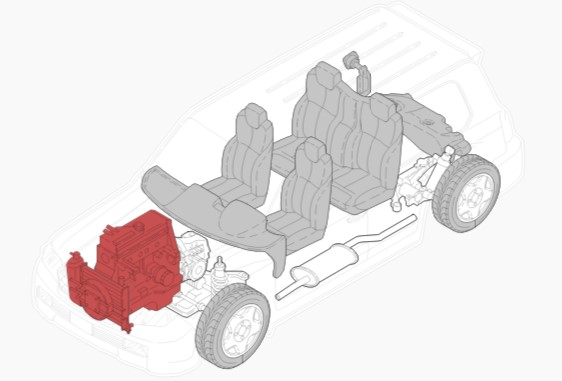
\includegraphics[width=0.65\linewidth]{images/cm1}
%	\caption{{\footnotesize {Компоновка \тс. Иллюстрация Audatex}}}
%	\label{ris:images/cm1}
%\end{figure}
%%%%%%%%%%%%%%%%%%%%%%%% КОНЕЦ ДЛЯ АВТОМОБИЛЯ
Свидетельство о регистрации  ВК № 384784 и паспорт самоходной машины и других видов техники ТС № 001742 содержит имеющие значения для производства исследования следующие    данные:

\begin{description}
%		
	\item[Марка, модель] -- KOMATSU FG15T-20
    \item[заводской номер машины] -- 661043
	\item[год выпуска ] -- 2007
	\item[тип машины] -- автопогрузчик колёсный
	\item[цвет машины] --  жёлтый-серый-зелёный
    \item[тип двигателя] -- бензиновый
    \item[модель и номер двигателя] -- К15-019305Х
    \item[мощность двигателя, кВт / л.с.] -- 27 / 36
    \item[конструкционная масса] -- 2720
    \item[габаритные размеры, мм] --  2300 / 1070 / 2030
    \item[дата выдачи свидетельства о регистрации машины] -- 08.08.2007 г.
    \item[дата выдачи паспорта самоходной машины и других видов техники] -- 24.05.2007 г.
    \item[собственник ТС ] -- ООО «Логистик-Юг» 
    \end{description}
\vspace{2mm}
\фотомасштаб{ттхдвигателя}{Технические характеристики двигателя \двигатель}{145mm}

\дварядом{1}{Погрузчик, аналогичный исследуемому \тс}{2}{Двигатель, аналогичный исследуемому \двигатель }

\vspace{3mm}
\par Согласно  записям  заказ-наряда № 252 от 04.10.2019 г.,  акта № 441 от 04.10.2019 г. и счёта на оплату № 449 от 04.10.2019 г.  специалистом ИП Войтенко В.А. на погрузчике, принадлежащему ООО «Логистик-Юг», были выполнены ремонтные работы  на общую сумму 115 409 рублей. В том числе: стоимость работ и услуг произведено на сумму 48 800 рублей, стоимость запасных частей составила 68 609 рублей (Рис. \ref{переченьдеталей}).    

\vspace{7mm}
\begin{figure}[H]
    \centering
    \includegraphics[width=1.01\linewidth]{foto/смета1}
%    \caption{}
%    \label{fig:}
\end{figure}
\begin{figure}[H]
    \centering
    \includegraphics[width=1.01\linewidth]{foto/смета2}
        \caption{Перечень работ, услуг и деталей к заказ-наряду 252 от 04.10.2019}
       {\footnotesize\label{переченьдеталей}}
\end{figure}

\begin{flushleft} 
    \hbox{% 
        \vrule\hspace{2.5mm}\parbox{1\textwidth}% 
        {\textit\small{\textit {Специалисты обращают внимание, что из приведённого перечня следует:  1) при выполнении ремонта ИП Войтенко В.А. в двигатель NISSAN К15 автопогрузчика KOMATSU FG15T-20 заводской номер 661043 было залито моторное масло 15W40, вопреки заводской инструкция «NISSAN» К15, К21, К25 бензиновый двигатель», предписывающей использовать для этого двигателя моторное масло 10W-30 (класс SJ); 2) список запасных частней не содержит болты головки блока цилиндров и термостат.(Рис. \ref{переченьдеталей})}}}}
\end{flushleft}


\subsection{Исследование погрузчика}
%\subsection{Исследование транспортного средства}
%
%Исследование автомобиля производилось экспертом с использованием производственных мощностей автообслуживающего предприятия дилерского сервисного центра в г. Краснодаре, ул. Аэропортовская, 4/1. При проведении осмотра присутствовали: \присутствовали. \\
%Автомобиль предоставлен частично разобранным: демонтирован поддон двигателя, вкладыши коленчатого вала, шатунные катушки зажигания, свечи зажигания.  Отдельно представлена пластиковая емкость, содержащая 3 литра масла из двигателя ТС \тс.
%На момент осмотра на автомобиле имеются повреждения переднего бампера снизу слева в виде задиров, крыло заднее правое  имеет царапины ЛКП, бампер задний справа имеет царапины ЛКП, имеется повреждение лобового стекла. Давление в шинах колес передней и задней оси 2.3 бар, шины BRIDGESTONE TURA NZA 225/55R17 97V
Исследование автопогрузчика KOMATSU FG15T-20 заводской номер 661043 производилось специалистами 25.02.2020 г. в условиях производственного крытого помещения при искусственном освещении по адресу: \местоосмотра\, в присутствии представителя ООО «Логистик-Юг», в лице генерального  директора Тарасова Андрея Ивановича. ИП Войтенко В.А. на осмотр не явился,  о месте и времени исследования уведомлен надлежащим образом.  На исследование автопогрузчик KOMATSU FG15T-20 заводской номер 661043 представлен в неработоспособном, частично разобранном состоянии (Рис.\ref{рис:видсправа}). Демонтированы радиатор системы охлаждения двигателя, крыльчатка вентилятора, кожух вентилятора.  Охлаждающая жидкость слита. Надписи, имеющиеся на автопогрузчике KOMATSU FG15T-20 заводской номер 661043, содержащие сведения о марке, модели заводском номере машины, годе  выпуска и цвете соответствуют записям регистрационных документов. Показание счётчика наработки на момент исследования составляет 6 472,7 моточаса (Рис.\ref{рис:vin},  \ref{рис:моточасы}). На автопогрузчике  имеется наклейка ООО "Югсервискар" с записью наработки моточасов на  16.01.2020 г., составляющая 6 463 моточаса и напоминанием о следующем техническом обслуживании при наработке 6 663 моточаса (Рис. \ref{рис:табличкато}).

%\subsubsection{Исследование ДВС погрузчика}

Уровень моторного масла в двигателе на момент исследования определён по масломерному щупу и находится значительно выше отметки "максимум". Масло коричневого цвета, со следами эмульсии (Рис. \ref{рис:уровень}, \ref{рис:уровень2}).

Образование эмульсии в моторном масле, появление густого белого дыма из выхлопной трубы, увеличение температуры двигателя  являются характерными признаками нарушения герметичности ЦПГ.

 Для разрешения вопросов исследования специалистами были осмотрены ранее демонтированные детали системы охлаждения и  частично разобран двигатель погрузчика. В процессе исследования специалистами производилась фото и видео съёмка этапов работ,  отобраны пробы моторного масла, выполнена проверка ранее демонтированных деталей системы охлаждения. Осмотром установлено: кожух и крыльчатка вентилятора радиатора системы охлаждения  исправны; радиатор системы охлаждения  конструктивно соответствует радиатору двигателя Nissan К15-019305Х;  радиатор герметичен,  внешних повреждений не имеет, передняя сторона радиатора чистая,  задняя сторона радиатора на отдельных участках имеет незначительное наслоение пыли и пуха,  следы масляной грязи отсутствуют,% внутренние поверхности радиатора покрыты плёнкой отложений тёмного цвета, 
трубки радиатора имеют удовлетворительную пропускную способность.   По совокупности признаков, радиатор находится в исправном состоянии, замена радиатора не требуется (Рис. \ref{рис:радивент}, \ref{рис:радиатор1}, \ref{рис:радиатор2}). 
Далее, для снятия головки блока цилиндров демонтированы:  генератор, впускной и выпускной коллекторы, отсоединены электрические разъёмы, крышка клапанов,  корпус термостата. Выявлено, что термостат в системе охлаждения двигателя  отсутствует (Рус. \ref{рис:корпустермостата}, \ref{рис:корпустермостата2}). Со слов представителя собственника автопогрузчика KOMATSU FG15T-20 заводской номер 661043, термостат был демонтирован специалистами ИП Войтенко В.А. во время ремонта. Причина, по которой термостат исключён из системы охлаждения неизвестна, в перечень деталей, подлежащих замене, термостат не включён. В каналах системы охлаждения содержится небольшое количество (остаточные следы) антифриза зелёного, слегка желтоватого цвета, жидкость прозрачная, без пены и загрязнений.  Свечи зажигания всех четырёх цилиндров имеют примерно одинаковый  слой сажевого осадка на изоляторе и боковом электроде.  
Для дальнейшей разборки двигателя произведён слив моторного масла   в подготовленные чистые пластиковые 5 литровые ёмкости. Согласно «Заводской инструкции» в двигателе NISSAN К15 должно быть 3,7 л моторного масла включая масло в масляном фильтре.   Однако, из масляной системы исследуемого двигателя  было слито более 6 л тёмной коричнево-серой эмульсии моторного масла и охлаждающей жидкости, что явно указывает на  утечку жидкости из системы охлаждения в масляную систему ДВС.  Дополнительным подтверждением попадания жидкости из системы охлаждения в систему смазки в процессе работы двигателя служит наличие  густого налёта сметанообразной эмульсии на внутренней поверхности  демонтированной  крышки клапанов. Металлическая стружка, мелкодисперсные металлические включения на дне поддона двигателя и в моторном масле отсутствуют.

Головка блока цилиндров двигателя \двигатель \, выполненная из алюминиевого сплава, штатно должна крепится к блоку цилиндров  при помощи 10-ти болтов. На исследуемом двигателе головка блока цилиндров крепится 9 болтами  и 1-й  шпилькой с двумя гайками, которая кустарным образом используется вместо штатного  болта между  1 и 2 цилиндрами (Рис. \ref{рис:головка}, \ref{рис:головка0}).

При снятии   газораспределительного механизма, специалисты отмечают, что болты крепления оси  коромысел откручиваются с меньшим, чем обычно усилием. Особенностью конструкции данного двигателя является нижнее расположение распределительного вала. Вследствие этого, связь между распределительным валом и коромыслами клапанов ГРМ осуществляется через штанги-толкатели. На поверхностях демонтированных штанг клапанов ГРМ присутствует слой эмульсии моторного масла и охлаждающей жидкости.  

Болты крепления крепления головки блока цилиндров откручиваются с небольшим усилием. Верхняя гайка на шпильке,  кустарным образом используемая вместо штатного болта крепления ГБЦ, имеет под собой разрушенную, сорванную резьбу (Рис. \ref{рис:гайканашпильке}, \ref{рис:гайка1}, \ref{рис:шпилькарезьбаторец}, \ref{рис:резьбашпилькиблок}). Данная шпилька откручивается с минимальным усилием, практически не затянута. Длина  открученной шпильки, начиная от нижней гайки, длиннее тела штатного болта,  шпилька изготовлена из мягкой стали, без термообработки (твёрдость материала шпильки ниже, чем твёрдость имеющихся болтов  головки блока цилиндров), очищенная от масла поверхность шпильки  цвета металла, характерного для оцинкованных металлических изделий. Торец шпильки имеет признаки обработки ручным инструментом (Рис.\ref{рис:торец}). 
Поверхность камеры сгорания, днища поршней, тарелки покрыты слоем  нагара сажевого цвета. Седла клапанов без повреждений, поверхности камер сгорания без признаков перегрева (Рис.\ref{рис:пробой1}). 
На исследуемом двигателе для уплотнения соединения блока цилиндров и головки блока цилиндров применена многослойная стальная прокладка (МСС-прокладка) с поверхностным эластомерным слоем. На прокладке между 1-2 и 2-3 цилиндрами имеют место характерные следы утечки газов между цилиндрами и утечки воды в масляный контур. Привалочные плоскости ГБЦ имеют разнонаправленные продольные вмятины (борозды, прощупываются пальцем), предположительно от воздействия на ГБЦ твёрдыми предметами. В отверстии  блока цилиндров, в которое была установлена шпилька, повреждена резьба.% Характерный для перегретого двигателя конденсат или признаки его образования между блоком цилиндров и головкой блока цилиндров отсутствует.

Измерение привалочной поверхности блока цилиндров показали отклонения от плоскости не более 0,03 мм. (Стандартная величина продольного прогиба 0,05 мм; диагонального 0,02 мм. Предельное значение деформации 0,1 мм для продольного и 0,04 мм для диагонального не превышено).  Измерение плоскости   поверхности  головки блока цилиндров показало значительный прогиб  между 1-2 цилиндрами от 0,10 до 0,15 мм, зазор  между 2-3 и 3-4 до  0,05 мм.  (Стандартная величина продольного прогиба 0,05; диагонального 0,02. Имеет место превышение предельно допустимого значения  деформации 0,1 мм для продольного и 0,04 для диагонального ). Таким образом, на исследуемом двигателе деформирована только привалочная плоскость головки блока цилиндров, поверхность блока цилиндров находится находится в допуске (Рис. \ref{рис:измерениеГБЦ}). 

%Исследование кривошипно-шатунного механизма, по согласованию с заказчиком исследования,  проводилось без разборки механизма.
Большое количество нагара на днищах всех поршней и в камерах сгорания. 
Рабочие стенки гильз блока цилиндров повреждений (задиров, царапин, наволакивания, наслоения металла) не имеют. Внутренние поверхности гильз сохранили следы заводского хонингования. Поршни в цилиндре расположены плотно,  с допустим зазором.  Измерением внутренних диаметров цилиндров установлено отсутствие отклонения сверх допустимых значений геометрии  цилиндров.  Максимальная разность диаметров на четырёх цилиндрах составляет не более 0,02 мм, что является допустимой величиной (нормальный диаметр гильзы двигателя К15  75.50 - 75.55 мм, предельный диаметр 75.70; внутренняя рабочая поверхность  гильзы может иметь эллипсность и конусность не более 0,1 мм и разницу между диаметрами не более 0,2 мм.).


\subsection{Анализ результатов исследования}

Значительный слой сажевого осадка на поверхности камеры сгорания, на изоляторе и боковом электроде свечей зажигания указывают на эксплуатацию двигателя  с частыми короткими пусками на топливной обогащённой смеси с 3-4х  кратным превышением стехиометрического коэффициента. На момент настоящего исследования  в системе смазки двигателя автопогрузчика KOMATSU FG15T-20 заводской номер 661043  объем жидкости почти в два раза (6 л. против 3.7 л) превышал допустимый (Рис. \ref{рис:эмульсия}).  Такое увеличение объёма жидкости в системе смазки ДВС могло образоваться вследствие нарушения герметичности сопряжения блока и головки блока цилиндров.    После демонтажа ГБЦ  обнаружено  локальное почернение  поверхностей прокладки ГБЦ со стороны головки блока между первым--вторым и вторым--третьим  цилиндрами и между первым--вторым со стороны блока цилиндров (Рис. \ref{рис:головка101}), (Рис. \ref{рис:блок1}). Подобные газовые утечки с почернением  описаны в литературе [16, 24, 25, 26] как основной индикатор недостаточного поверхностного давления \сноска{Под поверхностным давлением подразумевается сила на единицу площади поверхности контакта двух компонентов, например, между головкой блока цилиндров   и прокладкой головки блока цилиндров. В     противоположность прижимному усилию     поверхностное давление в разных частях     площади контакта не постоянно.} уплотнения или перегрева двигателя.  Возможными причинами недостаточного поверхностного давления уплотнения могут быть дефектные или вторично использованные болты крепления головки блока цилиндров, неправильная затяжка болтов, повреждения головки блока цилиндров и/или блока цилиндров, а также несоблюдение инструкций по сборке (Рис. \ref{рис:давлениенорма}, \ref{рис:давлениемало}).
Повреждение прокладки головки блока цилиндров возможно вследствие:

\begin{compactlist}
    \item [--] перегрева двигателя;.
    \item [--] деформации привалочных  плоскостей;  
    \item [--] нарушения затяжки болтов крепления головки блока цилиндров;
    \item [--] неудовлетворительного качества  прокладки ГБЦ.
\end{compactlist}


В большинстве случаев причиной, приводящей к повреждению прокладкой ГБЦ, является  перегрев двигателя [15, 16]. В результате перегрева возможно нарушение геометрии головки блока цилиндров или блока цилиндров, или головки и блока вместе взятых.  Как следствие, возникает разгерметизация внутренней полости со всеми вытекающими последствиями. Преимущественно, деформации подвергаются алюминиевые  головки блока цилиндров.

Другой причиной повреждения прокладкой ГБЦ является нарушение момента затяжки болтов. Негативное влияние оказывает как очень большое, так и малое значение момента. 

\subparagraph{Первая возможная причина - перегрев.}
В эксплуатации ДВС встречаются различные  причины перегрева двигателей [13, 19]:
1)	неисправности, вызывающие нарушение циркуляции ОЖ в системе (в том числе, неисправности термостата, насоса, загрязнение радиатора изнутри),
2)	неисправности агрегатов, нарушающие отвод теплоты из системы (в том числе, неисправности датчиков, вентилятора, загрязнение радиатора снаружи),
3)	утечки ОЖ из системы (в том числе, вследствие негерметичности от повреждения хомутов, шлангов, радиатора и т.д.).
Первые две группы причин имеют общий признак - нормальное количество ОЖ на момент начала повышения температуры в системе. В этом случае момент наступления перегрева двигателя, а также его развитие во времени контролируются с помощью указателя температуры на панели приборов, причём указатель покажет отклонение температуры от нормы при любой неисправности, входящей в указанные группы.
3-я группа представляет собой аварийный случай, когда из системы уходит рабочая жидкость. Это может существенно изменить режим работы системы вплоть до такого состояния, когда обычные методы контроля неприменимы.
Фактически речь идёт о перегреве, имеющем специфический характер, где специфика условий определяется, в 1-ю очередь, сочетанием чрезвычайно высокой температуры тех деталей, у которых утрачен контакт с ОЖ, со сравнительно более низкой температурой деталей, где такой контакт не нарушался. В случае, если датчик температуры оказывается вне жидкости из-за сильного падения ее уровня в системе,возможно существенное расхождение измеренной и действительной температуры, что  может стать причиной тяжёлых повреждений.\\
Конструкции системы охлаждения  исследуемого типа двигателей в настоящее время является самой распространённой, и
характеризуется следующим:
 
• система охлаждения герметичная, с принудительной циркуляцией, включает в себя одноходовый термостат с перепускным клапаном, поддерживающий установленную рабочую температуру ОЖ, наличие малого (снаружи или внутри двигателя, с помощью байпассного канала от выхода из головки до входа в насос) и большого (через радиатор) кругов циркуляции ОЖ, 
большой круг циркуляции управляется термостатом при постоянно открытом малом круге,

• насос ОЖ с приводом от коленчатого вала двигателя,

• вентилятор  для принудительного обдува радиатора в случае превышения температурой максимального заданного значения, управление включением вентилятора  по сигналу датчика температуры радиатора (Рис. \ref{схеатермостата}).


% TODO: схема термостата
\begin{figure}
    \centering
    \includegraphics[width=0.7\linewidth]{foto/схематермостата}
    \caption{ Система охлаждения традиционного типа с одноходовым термостатом: 1-отопитель, 2- двигатель, 3- термостат, 4- насос, 5- радиатор, 6- пробка, 7- вентилятор, 8- расширительный бачок, 9- байпассный канал малого круга циркуляции.А-малый круг циркуляции, термостат закрыт, Б-большой  круг циркуляции, термостат открыт}
    \label{схеатермостата}
\end{figure}

Во время работы двигателя при перегреве происходит нагрев ОЖ по той или иной причине до температуры кипения. При этом кипение начинается локально в рубашке охлаждения в зонах с наиболее нагретыми деталями - обычно это стенки камеры сгорания, выпускные каналы в ГБЦ. Далее кипение распространяется по объему жидкости - по мере разогрева деталей и самой жидкости. Фактически кипение жидкости создает паровую подушку между нагреваемой газами стенкой и ОЖ, препятствующую процессу отвода теплоты от стенок в жидкость.\\
Анализ имеющихся в литературе [13, 16, 19] данных позволяет указать основные признаки сильного и/или длительного перегрев двигателя в эксплуатации (в порядке увеличения интенсивности и длительности):\\
1.	Ослабление болтов ГБЦ.\\
2.	Деформация плоскости ГБЦ.\\
3.	Пластическая деформация прокладки ГБЦ, потеря герметичности, прорыв газов через нее.\\
4.	Загрязнение расширительного бачка маслом и нагаром, запах отработавших газов, разбрызгивание ОЖ в подкапотном пространстве.\\
5.	Деформация цилиндров.\\
6.	Задиры на поршнях в верхней части огневого пояса вследствие термического расширения днища и заклинивания поршня в цилиндре.\\
7.	Блокирование колец в канавках поршней вследствие задиров на поршне и цилиндрах от перегрева поршней.\\
8.	Задиры на краях юбок поршней от чрезмерного теплового расширения поршня, следы перегрева на внутренней поверхности поршней.\\
9.	Задиры в средней части цилиндров от юбки поршней.\\
10.	Плавление стенок ГБЦ у седел выпускных клапанов.\\
11.	Плавление верхней части поршня из-за нарушения охлаждения.\\
12.	Задиры на поршнях в верхней части огневого пояса вследствие попадания расплавленных частиц материала ГБЦ в зазор между поршнями и цилиндрами.\\
13.	Прочие признаки, в том числе, оплавление наконечников свечей зажигания, датчиков, впускного коллектора и других элементов, закреплённых на ГБЦ.\\


В процессе настоящего исследования на двигателе \двигатель\, погрузчика \тс\, обнаружено ослабление болтов ГБЦ, деформация плоскости ГБЦ и потеря герметичности прокладки ГБЦ.  Иные признаки, указывающие на перегрев двигателя отсутствуют. Напротив, исследуемое повреждение ДВС произошло при отсутствии термостата в системе охлаждения ДВС, т.е в принудительном режиме   циркуляции ОЖ по большому и малому кругу. Отсутствие повреждений элементов системы охлаждения при явном отсутствии повреждений радиатора, в совокупности с исключением термостата из системы охлаждения на исправном двигателе должны были привести не к перегреву, а напротив,  к увеличению времени прогрева двигателя до рабочей температуры вследствие необходимости нагрева большого объёма ОЖ с момента пуска двигателя. 
Исходя  из вышеизложенного, необходимо произвести анализ другой возможной причины возникновения неисправностей, а именно нарушение затяжки болтов крепления головки блока цилиндров.   
  
\subparagraph{Вторая возможная причина - нарушения затяжки болтов крепления головки блока цилиндров.}

Болты головки блока цилиндров являются конструктивным элементом присоединения ГБЦ, обеспечивающим необходимое общее усилие на прокладку ГБЦ. При любом рабочем режиме двигателя они должны обеспечивать необходимое прижимное усилие и его распределение по прокладке ГБЦ. Конструктивной особенностью двигателя \двигатель\, является алюминиевая головка блока цилиндров и  чугунный блок цилиндров. Так как линейный коэффициент температурного расширения алюминия практически  в 2 раза выше коэффициента теплового расширения чугуна ,  то и болты головки блока цилиндров должны удлиняться вместе с ГБЦ при нагреве и возвращаться обратно к исходному размеру при остывании.  Заворачивание болтов с определенным моментом затяжки и углом дозатяжки позволяет целенаправленно использовать характеристики болтов, при этом достигается очень маленький допуск усилия болта.  Для этого болты затягивают сверх предела текучести при растяжении до области пластической деформации. В двигателе \двигатель\, используются болты головки блока цилиндров с заводским артикулом  N11056-FY500.  Болт длиной 120 мм, 110 мм стержнем и 28 мм длиной резьбовой части М10*1,5, углом резьбы \угол{60} (Рис. \ref{рис:болты}).
     \сноска{Маркировка болтов изготовителя: рельефное нанесение на голове болта 9, обеспечивает усилие затяжки для резьбы М10х1,5 69.6-89.2 Нм.} 
Изготовитель двигателя \двигатель\, предписывает схему затягивания болтов ГБЦ, где помимо  приложения заданного момента усилия затяжки, равного 68.6 Нм, предполагается  достижение необходимого поверхностного давления  доворотом болта на угол  \угол{90}  \approx  \угол{92} с момента 19,6-23,52 Нм, (см. таблицу \ref{схемазатяжки}):
\vspace{2.5mm}
\begin{table}[H]
           {\small \begin{tabular}{c|c|c}
            \hline
            \textbf{n/n } & {\textbf{Момент затяжки болта ГБЦ, Нм}} & \textbf{Ремонттное воздействие} \\
            \hline
            1 & 19.6-23.52 & Временно затянуть \\
            \hline
            2 & 68.7 & Затянуть \\
            \hline
            3 & 0,0 & Ослабить \\
            \hline
            4 & 19.6-23.52 & Временно затянуть \\
            \hline
         %   5 & 68.7 & Затянуть \\
          %  \hline
            5 & $90^{\circ}$ \approx $92^{\circ}$ & Довернуть на угол \\
            \hline
    \end{tabular}}
    \caption{Схема затяжки болтов ГБЦ по данным изготовителя}
    \label{схемазатяжки}
\end{table}

\vspace{2.5mm}
  В исследуемом двигателе  болт ГБЦ между первым и вторым цилиндром  заменён стальной шпилькой М10х1,5. В месте установки шпильки наблюдаются повреждения прокладки головки блока цилиндров и наибольший прогиб привалочной плоскости ГБЦ.  По стандарту DIN 975,  выпускаются резьбовые шпильки  М10х1,5 длиной 1 и 2 м , с углом резьбы 35, 45 или 60 градусов. Серийно изготавливаются высокопрочные шпильки  М10х1.5 класса прочности  8.8 с углом \угол{60}. В данном случае, применена шпилька M10х1.5 с углом резьбы \угол{45}, класс прочности 4.8.  Однако, даже в случае применения шпильки М10 класса прочности 8.8 и углом резьбы \угол{60}, максимальное усилие затяжки могло составлять 45.1 (57.2) Нм, при необходимом усилии затяжки крепления головки блока цилиндров 68.7 нМ плюс дополнительный доворот на \угол{90}. Данному усилию затяжки с резьбой М10  соответствуют болты не ниже 10.9 класса прочности.\\ Таким образом, на основании изложенного, специалисты утверждают, что в случае замены штатного болта головки блока цилиндров серийной резьбовой шпилькой  попытка затянуть шпильку моментом 68.7 Нм приведёт к механическому разрушению резьбового соединения. В свою очередь,  затяжка болтов моментом 68.7 Нм с последующим ослабление до 0 Нм необходима для обжимки по месту  прокладки ГБЦ, так как используется многослойная стальная прокладка. Таким образом,во-первых,  установка прокладки ГБЦ будет произведена без должной обжимки, с нарушением требований изготовителя [22,23], а во-вторых различие физических свойств материалов болтов и шпильки ведёт к тому, что для этих деталей  предел текучести будет разный, как следствие различная сопротивляемость  действующим динамическим и ударным нагрузкам,  температурным циклами нагрев-охлаждение. \\
  
Следовательно, вследствие замены штатного болта крепления головки блока цилиндров ремонтной шпилькой, достижение равномерного  необходимого поверхностного давления  физически не представляется возможным. Как следствие - различия в эластичности болтового соединения, противодействиях динамическим и ударным нагрузкам, накоплении усталости от времени и циклов и поддержании внутреннего напряжения с течением времени.


% TODO: По первому вопросу
\повопросу{1. Какие неисправности имеет двигатель самоходной машины  KOMATSU   АВТОПОГРУЗЧИК  FG15T-20   2007 года выпуска, заводской номер 661043?}

В результате проеденного исследования специалистами установлено, что на момент  исследования  двигатель \двигатель \, \тс\, имел следующие неисправности:

\begin{itemize}
    \item 	отсутствует охлаждающая жидкость;
    \item   двухкратное превышение жидкости в системе смазки; 
    \item 	наличие в системе смазки двигателя жидкости из системы охлаждения;
    \item 	отсутствует термостат;
    \item 	для крепления ГБЦ к БЦ используется нештатный крепёж, болт головки блока цилиндров заменён шпилькой из мягкого метала, резьба 
    на шпильке сорвана;
    \item  не плотное прилегание прокладки блока цилиндров, не обеспечивающее необходимое уплотнение между блоком и головкой блока цилиндров;
    \item   в месте установки шпильки нарушена герметичность, что привело к  прорыву газов между первым и вторым цилиндром и попаданию жидкости из системы охлаждения в систему смазки. 
    \item 	головка блока цилиндров имеет нарушение привалочной плоскостности, превышающей допуск изготовителя  на участке между первым--вторыми вторым--третьим цилиндрами, имеет разнонаправленные продольные вмятины, глубиной более 0,1 мм, при этом, отсутствуют характерные признаки механической обработки привалочных плоскостей в процессе ремонта; 
    \item 	В блоке цилиндров повреждено резьбовое посадочное место болта крепления головки блока цилиндров. 
\end{itemize}


% TODO: По второму вопросу
\повопросу{2. Какова причина их возникновения?}

Как следует из исследовательской части, причиной возникновения неисправностей является недостаточное усилие сжатия прокладки головки блока цилиндров, вызванное  нарушением алгоритма разборки/сборки двигателя \двигатель\, погрузчика \тс. А именно, нарушение требований изготовителя по снятию/установке головки блока цилиндров.   При затягивании болтов головки блока цилиндров не был соблюден порядок и моменты затягивания болтов ГБЦ, следствием чего явилось повреждение одного из болтов крепления головки блока цилиндров и соответствующего ему резьбового посадочного места в блоке цилиндров. Далее, при сборке двигателя, были применены бывшие в употреблении болты крепления головки цилиндров, один из которых был заменен на кустарно изготовленную шпильку из мягкого металла с иными прочностными, упругими свойствами.  В процессе эксплуатации, через очень непродолжительное время, под воздействием циклических динамических, температурных и ударных воздействий,  обусловленных рабочим циклом двигателя внутреннего сгорания, шпилька растянулась, крепление шпилькой ослабло, произошло уменьшение прижимного усилия между головкой блока цилиндров и блоком цилиндром в области установки вышеуказанной шпильки, нарушилась герметичность сочленения блока и головки блока цилиндров, начался прорыв газов из камер сгорания между первым и вторым цилиндром, локальное кипение охлаждающей жидкости на раскалённых поверхностях камеры сгорания, нарушение теплового режима двигателя, смешивание охлаждающей жидкости с моторным маслом, деформация головки блока цилиндров под воздействием циклических сжимающих усилий  горения топливной смеси, динамических и температурных нагрузок. 

Отсутствие термостат  в системе охлаждения, и рекомендации организации, производившей ремонт погрузчика о необходимости замены радиатора можно объяснить попыткой ремонтников  восстановить тепловой режим ДВС, ошибочно полагавшим, что неисправность ДВС вызвана неисправностями элементов системы охлаждения двигателя.

Необходимо отметить, что после исследования ДВС,  была произведена проверка головки блока на отсутствие трещин.  Трещины не обнаружены. После механической обработки привалочной плоскости головки блока цилиндров, (шлифовки со снятием 0,06 мм материала) (Рис.\ref{рис:ремонт}), восстановлением повреждённой резьбы в блоке, заменой болтов крепления головки блока цилиндров неисправности двигателя \двигатель\, погрузчика \тс\, были полностью устранены. 


% TODO: По третьему вопросу
\повопросу{3. Причина выхода из строя вышеназванного двигателя  имеет производственный или эксплуатационный характер?}

При разрешении данного вопроса специалисты понимают термин "эксплуатационный" в контексте вопроса   как период использования погрузчика по назначению. Под термином "производственный характер" специалисты понимают период изготовления.  Период ремонта относится ко всему периоду эксплуатации агрегата.  Так как причиной выхода из строя двигателя \двигатель \, погрузчика \тс\, является ремонт, выполненный с нарушениями требований изготовителя, то причина выхода двигателя из строя должна быть отнесена к эксплуатационному характеру.  


% TODO: По четвертому вопросу
\повопросу{4. Могли ли имеющиеся неисправности двигателя \двигатель\, погрузчика \тс\,  возникнуть вследствие капитального ремонта?}

Понятие "ремонт" изложено в <<Положение о техническом обслуживании и ремонте подвижного
состава автомобильного транспорта>>, комплекс основных технологических ремонтных воздействий, характеризующих типовые процедуры выполнения различных видов работ по ремонту, представлен в документе «Рекомендации. Технологическое содержание услуг по ТО и ремонту автомототранспортных средств. Система сертификации ГОСТ Р. Система сертификации услуг по техническому обслуживанию и ремонту автомототранспортных средств». Р 3112199-0395-00. базовая и основные детали требуют ремонта с полной разборкой агрегата. Агрегат ТС направляется на капитальный ремонт или подлежит замене по следующим критериям:\\
базовая и основные детали требуют ремонта с полной разборкой агрегата;
работоспособность агрегата не может быть восстановлена по техническим причинам или ее восстановление путем проведения текущего ремонта экономически нецелесообразно.
Для двигателя внутреннего сгорания базовой деталью является блок цилиндров, основными деталями являются: головка блока цилиндров, коленчатый вал, маховик, распределительный вал.
Имеющиеся неисправности двигателя \двигатель \, погрузчика \тс\, явились результатом разборки/сборки его двигателя,  следовательно имеющиеся неисправности могли возникнуть вследствие его капитального ремонта. 


\vspace{2.5mm}
\section{Выводы}

\begin{enumerate}
	\item \textbf{ На момент  исследования  двигатель \двигатель \, \тс\, имел следующие неисправности:
\begin{itemize}
    \item 	отсутствует охлаждающая жидкость;
    \item   двухкратное превышение жидкости в системе смазки; 
    \item 	наличие в системе смазки двигателя жидкости из системы охлаждения;
    \item 	отсутствует термостат;
    \item 	для крепления ГБЦ к БЦ используется нештатный крепёж, болт головки блока цилиндров заменён шпилькой из мягкого метала, резьба 
    на шпильке сорвана;
    \item  неплотное прилегание прокладки блока цилиндров, не обеспечивающее необходимое уплотнение между блоком и головкой блока цилиндров;
    \item   в месте установки шпильки нарушена герметичность, что привело к  прорыву газов между первым и вторым цилиндром и попаданию жидкости из системы охлаждения в систему смазки. 
    \item 	головка блока цилиндров имеет нарушение привалочной плоскостности, превышающей допуск изготовителя  на участке между первым--вторыми вторым--третьим цилиндрами, имеет разнонаправленные продольные вмятины, глубиной более 0,1 мм, при этом, отсутствуют характерные признаки механической обработки привалочных плоскостей в процессе ремонта; 
    \item 	В блоке цилиндров повреждено резьбовое посадочное место болта крепления головки блока цилиндров. 
\end{itemize}    
 }
    \item \textbf{Причиной возникновения неисправностей является недостаточное усилие сжатия прокладки головки блока цилиндров вследствие нарушения технологии сборки двигателя}
    	\item \textbf{Причиной выхода двигателя из строя является неквалифицированный ремонт двигателя \двигатель\, погрузчика \тс, проведенный в период эксплуатации погрузчика.}
    \item \textbf{Имеющиеся неисправности могли возникнуть вследствие его капитального ремонта.}
\end{enumerate}
\vspace{15mm}
\relax


%\vspace{20mm}

\noindent {Специалист, инженер-механик}\hfill    {   Фефелов С. Л.}\\
{Специалист, инженер-физик}\hfill           { Мраморнов А.В.}

\vspace{15mm}
%\noindet{\footnotesize  Страниц документа \pageref{LastPage} }
\pagebreak

\begin{center}
 \textbf{{\Large    ФОТОТАБЛИЦА ПОВРЕЖДЕНИЙ}}
\end{center}

%\фото{}{}
%\дварядом{}{}{}{}
\фото{видсправа}{Погрузчик \тс\, вид справа. Состояние погрузчика на начало осмотра 25.02.2020}

\фото{vin}{Маркировочная табличка, установленная на исследуемом погрузчике \тс}
\фото{моторсобран}{Вид сверху на моторный отсек погрузчика \тс }
\фото{моторраз1}{Моторный отсек погрузчика \тс, клапанная крышка снята}
\фото{головка0}{Головка блока со снятой крышкой. Стрелка указывает на нештатный крепеж головки блока}
\фото{головка2}{Головка блока со снятой крышкой. Стрелка указывает на нештатный крепеж головки блока}
\дварядом{моточасы}{Наработка на момент осмотра 6472.7 моточасов}{табличкато}{сервисная табличка с указанием значения следующего сервисного обслуживания при наработке 6663 моточаса}
\дварядом{уровень}{контрольная линейка масломерного щупа}{уровень2}{Уровень моторного масла значительно выше допустимого}
\дварядом{эмульсия}{Слитое из ДВС моторное масло. Цвет эмульсии}{эмульсия2}{Клапанная крышка. Вид изнутри. Поверхность покрыта эмульсией}
\фото{радивент}{Радиатор ДВС, кожух и крыльчатка}
\дварядом{радиатор1}{Поверхность радиатора со стороны ДВС}{радиатор2}{Внешняя сторона }
\дварядом{корпустермостата}{Посадочное место термостата}{корпустермостата2}{Патрубок термостата}
\фото{болтишпилька}{Штатный болт ГБЦ и кустарноизготовленная шпилька}
\фото{торец}{Торец шпильки. Красной стрелкой отмечены заусенцы, желтыми стрелками следы обточки торца ручным инструментом}
\фотомасштаб{шпилькарезьбаторец}{Сорванная резьба шпильки со стороны контрогайки}{150mm}
\фотомасштаб{резьбашпилькиблок}{Резьба шпильки со стороны блока}{150mm}
\фото{гайканашпильке}{Нештатный крепеж головки блока цилиндров}
\фото{гайка1}{Нештатный крепеж головки блока цилиндров}
\фото{блок1}{Привалочная плоскость блока цилиндров}
\фото{головка101}{Привалочная плоскость головки блока цилиндров}
\фото{пробой1}{Поверхность головки блока со следами прорыва газов и охлаждающей жидкости
}
\фото{пробой2}{Поверхность головки блока со следами прорыва газов и охлаждающей жидкости}
\фото{пробой3}{Поверхность блока цилиндров со следами прорыва газов и охлаждающей жидкости}
\фото{прокладка}{Прокладка ГБЦ}
\фото{измерениеГБЦ}{Деформация более 0,1 мм}
\фото{наборболтов}{Крепежные компоненты головки блока цилиндров исследуемого двигателя}
\фото{грязьврезьбе}{Резьбовая часть головки блока цилиндров исследуемого двигателя}
\фото{головка100}{Вероятная трещина в головке блока цилиндров}
\фото{головка3}{Вероятная трещина в головке блока цилиндров}
%\фото{}{}
%\фото{ремонт}{}
%\фотомасштаб{}{}{}
\дварядом{давлениенорма}{Поверхностное давление при штатной установке}{давлениемало}{Поверхностное давление со слабой шпилькой}
\фото{ремонт}{Механическая обработка}
%\дварядом{}{}{}{}
%\imgh{160mm}{1}{2}